\section{Progettazione}

\subsection{Obiettivi}
Nello sviluppo del sito il gruppo si è imposto il conseguimento dei seguenti obiettivi:
\begin{itemize}
	\item \textit{Separazione tra struttura/contenuto, presentazione e comportamento}: il suo
	raggiungimento comporta una maggior facilità nel soddisfare anche gli altri obiettivi. I
	contenuti del sito e la loro struttura devono essere separati dalla parte di presentazione grafica e
	dalla parte dinamica dello stesso. A tale scopo si è deciso di separare il sito nel seguente modo:
	\begin{itemize}
		\item Struttura e contenuto: le informazioni sono codificate in pagine HTML;
		\item Presentazione: si è data un'impostazione grafica al sito tramite fogli di stile CSS;
		\item Comportamento:
		\begin{itemize}
			\item Lato client: script JavaScript;
			\item Lato server: script PHP.
		\end{itemize}
	\end{itemize}
	\item \textit{Accessibilità}: il sito deve poter essere navigabile dal maggior numero di utenti
	possibile, compresi quelli con disabilità visive e/o motorie. Le misure prese a tale scopo saranno
	riportate successivamente;
	\item \textit{Flessibilità}: il sito deve poter essere consultabile da varie tipologie di
	dispositivi. In particolare è essenziale garantire all'utente la possibilità di svolgere tutte le
	operazioni da smartphone, al fine di rendere l'esperienza utente più agevole possibile.
\end{itemize}

\subsection{Layout}
Per il layout del sito è stato scelto un \textit{ZigZag Layout} il quale si adatta bene al contesto in
quanto presuppone che l'utente legga le informazioni da sinistra verso destra, cosa a cui gli utenti
del sito sono culturalmente abituati, se non altro la quasi totalità.\\
\\
Il layout del sito si contraddistingue innanzitutto per la presenza di un header, che è sempre ancorato
sul lato superiore della finestra in modo da avere i link principali sempre a portata di mano, e di un
footer collocato alla fine di ogni pagina.\\
\\
Il corpo principale della maggior parte delle pagine è invece stato pensato come un insieme di
container dove ognuno di essi corrisponde ad una sezione della pagina, e sono caratterizzati da un titolo
e da un'insieme di subcontainer che sarebbero il contenuto di quella sezione.\\
\\
Siccome la maggior parte delle unità di misura di grandezza utilizzate sono relative, l'interfaccia scala
a seconda della dimensione del font impostata e dello schermo.\\
\\
Rispetto allo schermo di un computer, oltre ad essere più piccolo lo schermo di uno smartphone è
fatto per essere utilizzato in modalità potrait piuttosto che in modalità landscape. Occorre quindi che
il sito si adatti a queste differenze. Il layout del sito si trasforma quindi in un \textit{single
column layout}. Parlando delle differenze, in primo luogo il sito in versione mobile presenta un header
che mostra oltre al logo della pizzeria esclusivamente un'icona ad hamburger al cui click sarà possibile
mostrare/nascondere l'elenco delle voci. Inoltre, a causa dello spazio ridotto, il titolo di un
container in modalità mobile viene spostato in alto.
\newpage
\begin{figure}[H]
	\centering
	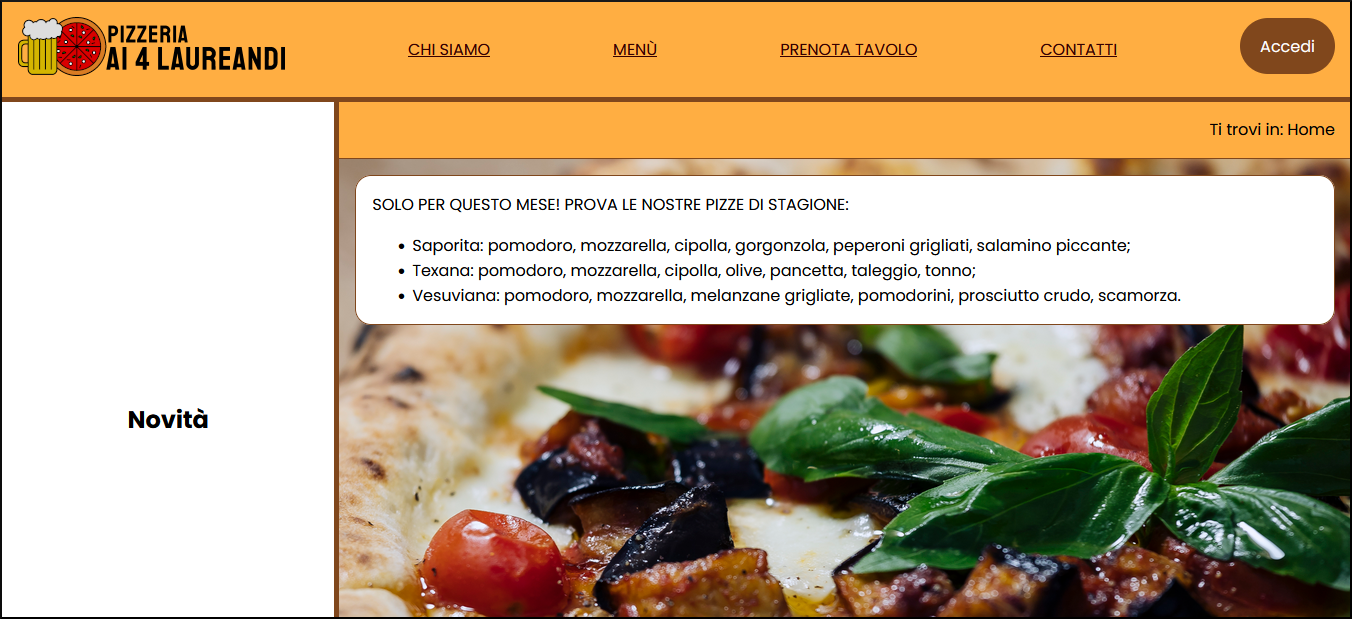
\includegraphics[scale=0.25]{resources/screenshot_index.png}
	\hspace{1cm}
	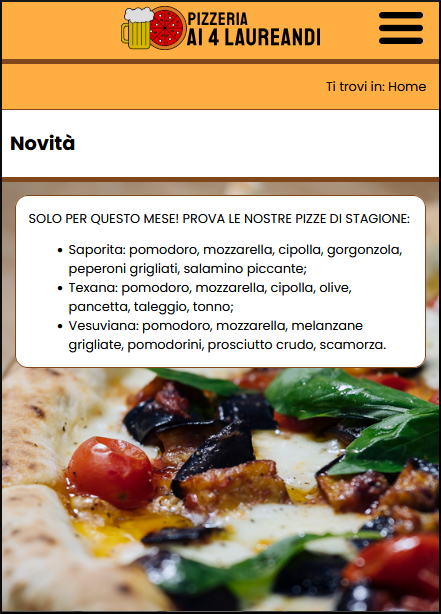
\includegraphics[scale=0.5]{resources/screenshot_index_mobile.png}
	\caption{Pagina principale del sito}
\end{figure}
\begin{figure}[H]
	\centering
	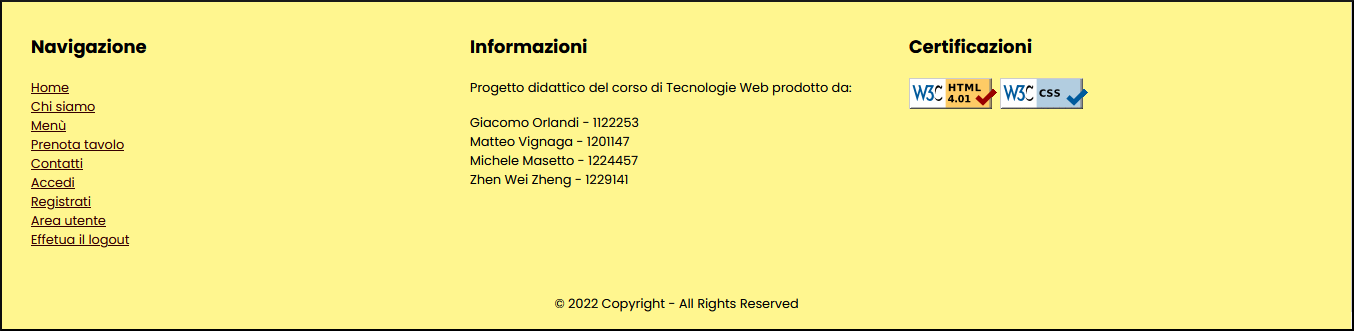
\includegraphics[scale=0.5]{resources/footer.png}
	\caption{Footer delle pagine del sito}
\end{figure}

\newpage
\subsection{Accessibilità}
Si è prestata particolare attenzione all'accessibilità del sito. A tal riguardo sono state prese le
seguenti misure:
\begin{itemize}
	\item Aggiunta di un testo alternativo alle immagini;
	\item Assegnazione di ogni parola che è contenuto alla sua lingua di appartenenza;
	\item Utilizzo di uno schema di colori che abbiano un buon livello di contrasto tra di loro ma
	che allo stesso tempo non diano fastidio durante la navigazione. Tale schema è anche semplice,
	ossia con pochi colori, per essere coerenti e favorire la creazione di una mappa mentale;
	\item Utilizzo di un font chiaro e semplice;
	\item Aggiunta di un \textit{breadcrumb} che indichi la posizione attuale all'interno del sito per
	evitare il disorientamento dell'utente;
	\item Utilizzo di una struttura del sito poco profonda in modo che ogni pagina sia raggiungibile
	partendo da quella principale con non più di tre click;
	\item Utilizzo di attributi \textit{ARIA} per fornire maggiori informazioni allo screenreader;
	\item Utilizzo dell'attributo \texttt{tabindex}, e del tag \texttt{fieldset} nei form;
	\item Come richiesto dalle \textit{WCAG}, utilizzo di due colori diversi per i link visitati e non,
	i quali per convenzione sono il blu ed il rosso;
	\item Adozione di un design del sito web responsive, ossia che si adatti elegantemente
	al dispositivo utilizzato.
\end{itemize}
\begin{figure}[H]
	\centering
	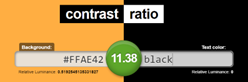
\includegraphics[scale=1]{resources/contrast_1.png}
	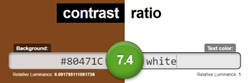
\includegraphics[scale=1]{resources/contrast_2.png}
	\caption{Livello di contrasto tra i colori di background e del font}
\end{figure}
\begin{figure}[H]
	\centering
	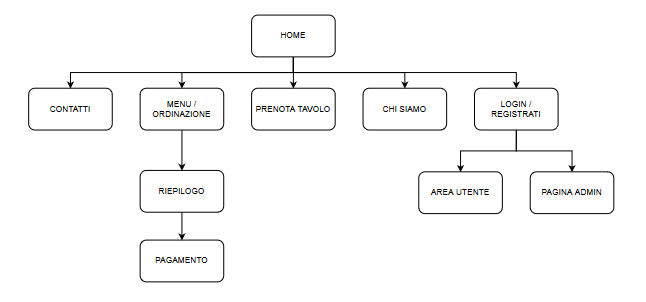
\includegraphics[scale=0.85]{resources/hierarchy.png}
	\caption{Gerarchia del sito.\\Si può notare che il grafo ad albero risultante
	possiede un'altezza pari a 3.}
\end{figure}